
\subsection{Product perspective}
\subsubsection{Internal structure}
\hspace{\parindent}The proposed system uses an application on the server side that is connected with the APIs to the Android or the iOS app on the phone.

The way of communication between the parts of the system and logic behind the system is presented in the following figure:
\begin{figure}[!htb]
\centering
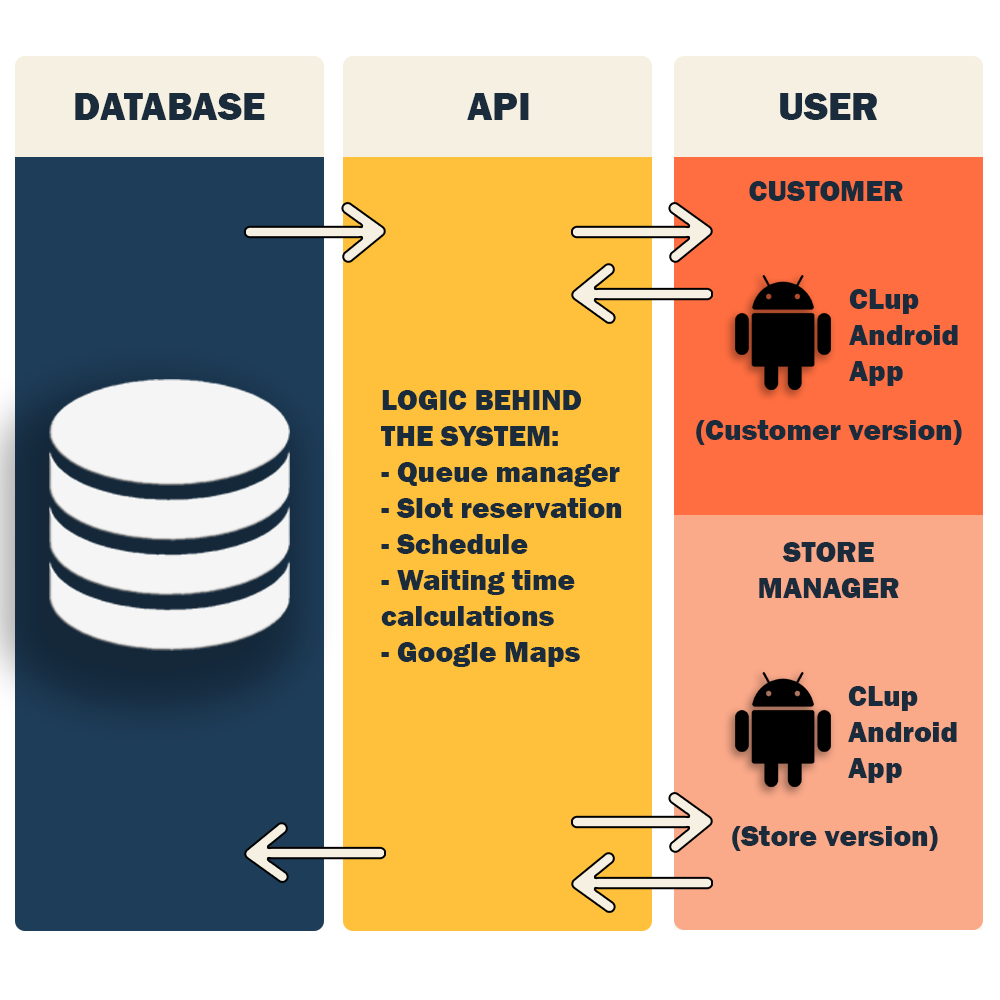
\includegraphics[width=\textwidth]{Images/DB_API_USER.png}
\caption{\label{fig:dbapiuser}\textbf{Internal structure of the system}}
\end{figure}
\newpage

The main part of the logic behind the system is on the server side. All the data taken from the users is stored in the database and all the data that users request, like stores' working hours, location, and available time slots, are also taken straight from it.

Since there is no need for users to have accounts, their personal data is not permanently stored in the database, therefore allowing users to use the app quickly and safely.

API is used to do all the work in between. Calculating waiting time, slot reservation, scheduling, queue management, and calculating distance is done based on the request by the user and with using the data provided by the database. 

Another part of the app is the store manager version, which requires login to connect a store manager to the specific store, so he/she can manage the influx of people to and from the store.

\paragraph{State chart diagrams}\hfill \break

\hspace{\parindent}Core functioning of the system is shown in this chapter using the state chart diagrams. These are simplified representations of the process that is happening during the most basic functionalities of the application and the system. Following state charts will be further explained and deepened through other diagrams in the following chapters. 

\begin{figure}[!htb]
\centering
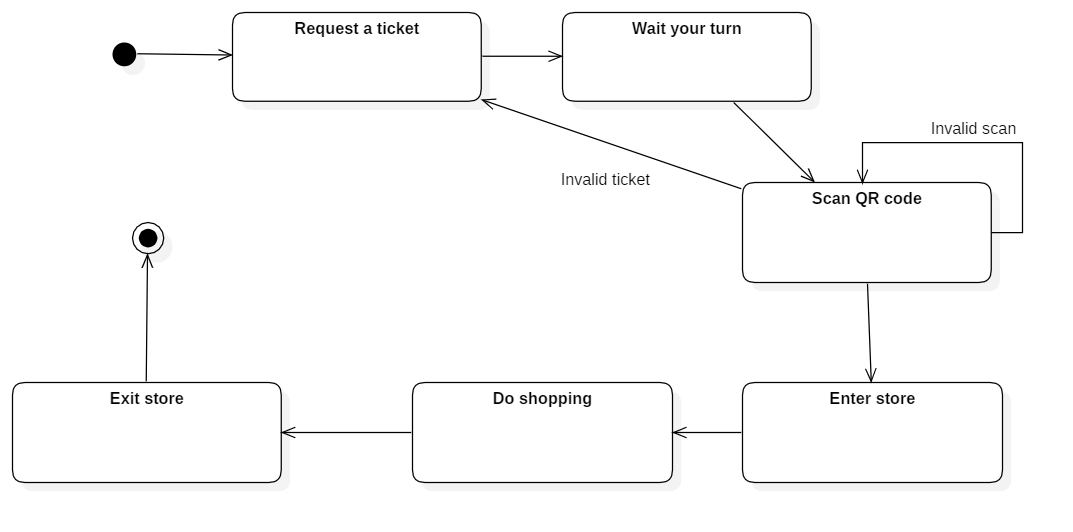
\includegraphics[width=\textwidth]{Images/StatechartDiagram1_RequestAndScan.png}
\caption{\label{fig:statechart1}\textbf{State chart diagram 1 - Request and scan}}
\end{figure}

\hspace{\parindent}\textbf{State chart 1} represents the most basic function of the CLup app - requesting and using a ticket. This diagram can be used both for the ticket request through the app or for taking the ticket from the printing machine. The mechanism works the same way. Once the ticket has been acquired by the customer, and the ticket's number gets called (either by the store manager or by the screen that shows the queue), the user must enter the store and present the ticket on his way in. The ticket will then be scanned and either accepted or denied by the store manager. After successfully entering the store, the customer can do the shopping and exit the store normally.  

\begin{figure}[!htb]
\centering
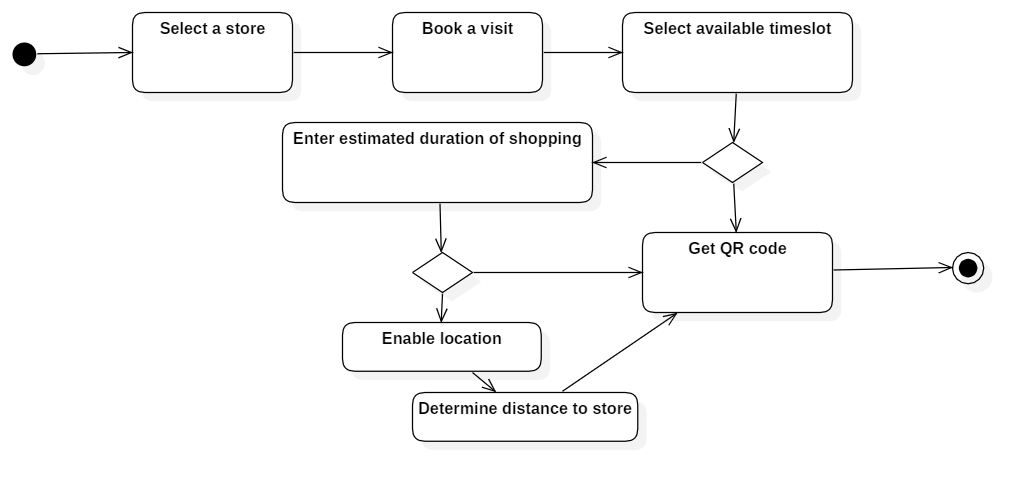
\includegraphics[width=\textwidth]{Images/StatechartDiagram2_BookAVisit}
\caption{\label{fig:statechart2}\textbf{State chart diagram 2 - Book a visit}}
\end{figure}

\hspace{\parindent}\textbf{State chart 2} shows the usage of the app's second feature - "Book a visit". This can be done exclusively through the app and it's not possible to do it in person. Booking a visit is aimed for people who have less time to wait in the line and is projected to be the most effective way of stopping any additional virus spreading, as there will be less people in front of the stores at the same time. The customer must select a store and an available timeslot through the app. The customer will then be presented with a ticket that can be used only during that timeslot and in that specific store which customer has specified. Customers also have an option of entering estimated duration of shopping as well as allowing the app to access location services of the device, which would then be used to calculate the full duration of the customer's visit to the store. This would not only help the customers, but also help regulate the traffic in stores. However, these two options are optional as they slow down the reservation process and acquire confidential information from the customers, which we want to avoid doing if not needed.

\newpage

\begin{figure}[!htb]
\centering
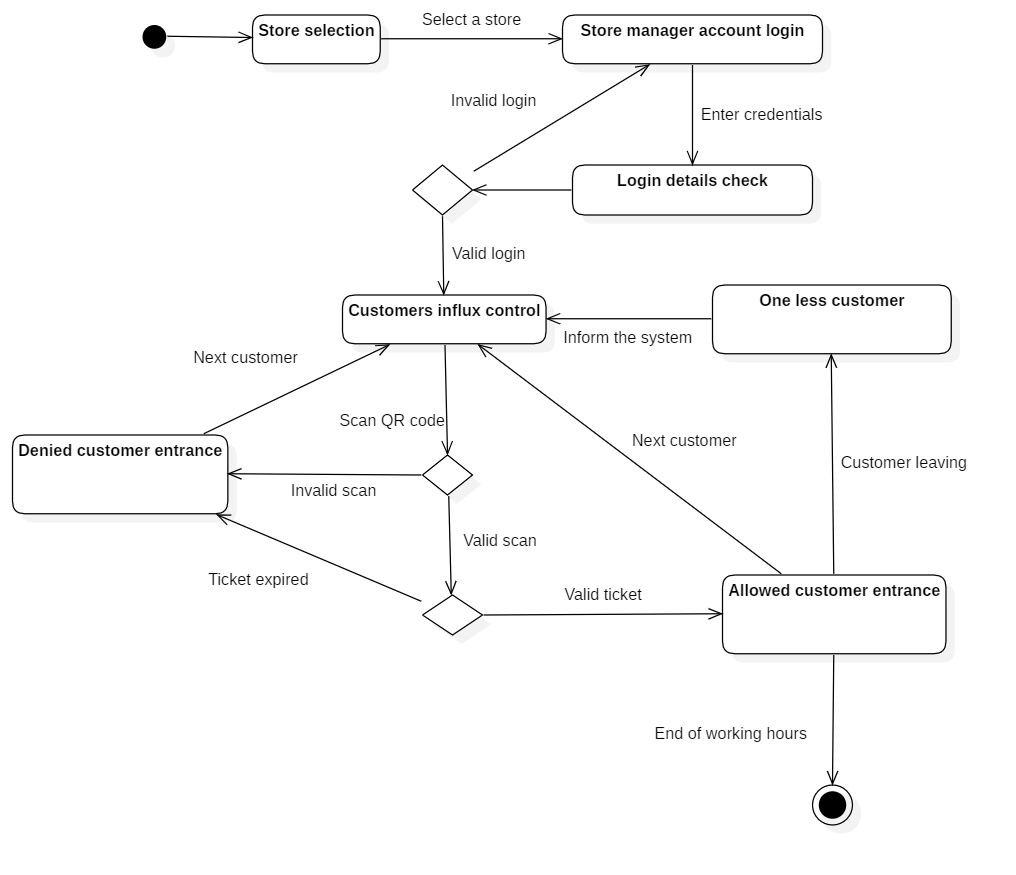
\includegraphics[width=\textwidth]{Images/StatechartDiagram3_StoreManager}
\caption{\label{fig:statechart3}\textbf{State chart diagram 3 - Store manager}}
\end{figure}

\hspace{\parindent}\textbf{State chart 3} describes the flow of the whole application usage for the store manager. Since every store manager is connected to a specific store that is in the system, it must provide the login details, which will be given during the store registration process. This diagram also shows how the store manager can control the influx of people to the store, simply by scanning their tickets' QR code when a customer enters and pressing the button when a customer exists. That way the store manager can keep the store under capacity at all times and make sure that no customer with an invalid ticket can enter the store.

\newpage

\subsubsection{Scenarios}

\textbf{Scenario 1}

\hspace{\parindent}During the COVID-19 pandemic the government has forbidden unnecessary trips outside of the living space, therefore only allowing people to go to the stores to buy groceries. Among the measures, the government has also allowed only up to 60 people in closed spaces. This has created a problem since the only place people can go is the store and there are often a lot of people waiting outside in line and by doing so, spreading the infection. The store owner decided to use CLup system to reduce the number of people outside of the store. He installed a small screen just inside the store so that the people can see the number displayed through the glass. He also put up a small printing device for the tickets as well as a store manager at the entrance so that the influx of people can be controlled. He also gives 5\% discount to everybody who uses CLup app by scanning their QR code at the cash register. This way he encourages people to use the app and not come to the store prematurely, so that the infection would not spread. This can also increase the profit a store makes since a lot of people would decide to go to the other nearby store if the line is too big. The lines have now been reduced and people can also make reservations so that they know exactly when they are going to be able to enter the store without waiting. \break

\textbf{Scenario 2}

\hspace{\parindent}Esselunga, one of the biggest supermarket chains in Italy, has a problem in their stores. Every working day of the week they have so called "rush hours" between 11 and 13, which is lunch time, and between 16 and 18, right after people finish their work. 
Because of the new restrictions, they are unable to allow everybody to go in which results in people going to the other stores and not waiting for their turn, since they do not have that much time. Every Esselunga store in Milano has therefore started using the CLup system. All Esselunga stores are put by the administrators in the system, along with their addresses and working hours. This way it will be easier for the users to find the exact Esselunga store they are looking for.  
Now customers can either reserve their spot in advance and plan their quick shopping accordingly, or just request a ticket when they are leaving their working space, so their waiting time is minimal. Both the stores and users have better shopping experience. \break


\textbf{Scenario 3}

\hspace{\parindent}A small store right next to the university and student housing area is having issues with too many students going to the store at once. Even though the store is only 50m away from the student housing, the students that are stuck in line decide to wait outside of the store and hang out with other students, therefore spreading the disease. The store owner has introduced the CLup system and completely disallowed people from entering the store without using the app. This way, students can easily make reservations and come to the store at a certain time, as well as just take a virtual ticket and come just a minute or two before it is their turn to enter. Since nearly every customer is a student and all of the students have access to the smartphones and Internet, the store owner hasn't lost any profit, and the students can now go to the store without waiting in line and risking getting the disease from one of their colleagues. \break

\newpage

\textbf{Scenario 4}

\hspace{\parindent}Ludovico is an elderly citizen fighting diabetes. Although not as physically capable as he once was, he still goes for a long walk twice a week to and from a grocery store in the neighborhood. Such a physical activity helps him keep his blood sugar levels low, keeping a healthy body as well as the mind. Because of the new government recommendations, he would often have to wait in line in front of the grocery store. In fear of catching the virus, he slowly stopped his weekly routine, ordering his supplies online. As time passed, he started noticing that he tires more easily and that his blood sugar levels were rising. Luckily, his grandson introduced him to the CLup application which allows him to rebuild his old habit, while minimizing the health risks. As he knows exactly how much it takes him to get to the store, he uses the "book a visit" feature and indicates the time he wants to be able to enter the store. \break

\textbf{Scenario 5}

\hspace{\parindent}Umberto is a hard-working middle-aged man, with two children and a loving wife. Although content with his current life situation, he often finds himself balancing between order and chaos. Work from 9 to 5, late lunch, or early dinner, then watching over the children while his wife is away. As she does not drive a car, he also has to fit in grocery shopping in his schedule. While all was in order before the pandemic, the new restrictions brought long lines in front of stores and often pushed his schedule into chaos. His problem was solved by switching to a store using the CLup application. He can now "book a visit" days before his planned trip to the grocery store and be certain that he will not have to wait long lines to get in. 

\newpage

\subsection{Product functions}
\hspace{\parindent}Functions of the final product should provide easy and accessible use for everyone, regardless of their experience and knowledge regarding technology and smartphones. 

These functions are mentioned on several places in the document, but their most thorough explanation can be found here.

\subsubsection{Generating a scannable QR code}

\hspace{\parindent}The most important part of the system. It must be able to generate a QR code quickly and responsively on the screen that replaces a real-life ticket. By generating this code, it should also "insert" the virtual ticket into the current ticket queue that is interpolated together with the real-life tickets, which are handed out at the store entrance. This code should remain visible in the application until it expires, so even if the user exits the application it does not get lost. No additional data nor any permissions are needed from the user to get the code. Generation request of the QR code is done by pressing a single button that is presented on the main screen of the application, so that even the less experienced users have no trouble generating the QR code. 
\subsubsection{Managing available shopping time slots}

\hspace{\parindent}
To support "book a visit" function, the system must maintain a schedule that is specific for each store. This means reserving a specific timeslot up front so that the user can just come to the store without generating a ticket in advance. However, the ticket still needs to be generated and inserted into queue in real-time. This part is to be done by the system itself and without any help of the user. The QR code must remain active until the specific time slot has passed. The system will insert the virtual ticket in the queue at the right moment either by using the average buying time or by  temporarily reducing the maximum amount of people that are allowed to be at the store, so that a specific slot is reserved for the user.

\subsubsection{Calculating average waiting time}

\hspace{\parindent}The system needs to be able to calculate average waiting time if the user is to take the ticket at that specific moment. This can be done by calculating the average shopping time in a certain day or time of day and multiplying it with the number of customers that are currently waiting in the queue. While this will not provide a perfect estimation, since it is possible that every customer shops for a lot longer or a lot shorter time, the deviation should not be off by a lot. By doing this we would ensure that there are no crowds in front of the stores as the customers would be prompted to arrive only when there are a couple of minutes until their turn. This part of the system should also provide notifications for the virtual ticket holders and inform them of how many customers are currently in front of them, and therefore how many minutes until they will be able to enter the store. 

\subsubsection{Calculating time needed to get to the store}

\hspace{\parindent}By providing their location, which has to be allowed by the user, the system can calculate the exact amount of time that user needs to get to the store. This is done by using one of the Google Maps APIs which allow the distance calculation of two specific locations as well as the time needed to get from one point to another. Together with the estimated shopping time provided by the user, this would allow the user to get the exact amount of time needed to make a shopping trip. While this function has no advantages to the effectiveness of the system itself, we believe that it is an important function for the user, and it would make the usage of the application much more enjoyable experience.

\newpage

\subsection{User characteristics}
\hspace{\parindent} There are four different categories of users in this application:

\subsubsection{User}
\hspace{\parindent}A person using the CLup application, not necessarily registered. The person can request to be queued in line, get an approximation of the wait time, and get updates on the estimated time left until their number is called. Furthermore, the person can request to inspect and reserve available time slots for the "book a visit" feature during which they can also indicate the estimated visit duration. 
\subsubsection{Store manager}
\hspace{\parindent}An employee of the grocery store that uses the CLup application in charge of monitoring and controlling the influx of customers of the store. The person scans the QR code of incoming customers to prevent irregularities and registers their exit time (specific information about which customer exactly is exiting is not necessary as this feature is used only for calculating wait time statistics). The person uses a different UI from an ordinary user and their credentials are added to the system directly through installation. 
\subsubsection{System manager}
\hspace{\parindent}An employee of CLup in charge of maintaining and updating the application. The person has administrative authority in the application setup during the system's installation. 
\subsubsection{Physical customer}
\hspace{\parindent}A person that for some reason is unable to line-up through the CLup application, and therefore must take a physical ticket from the printer. The person can take the ticket with minimal physical contact and wait until their number is called by the store manager. 

\newpage

\subsection{Assumptions, dependencies and constants}
\subsubsection{Assumptions}
\textbf{Domain assumptions}

\begin{itemize}
	\item[\textbf{D1}]The store manager's username must be unique. 
	\item[\textbf{D2}]The registered store manager's password secure. 
	\item[\textbf{D3}]The user's device provides accurate GPS information. 
	\item[\textbf{D4}]The system can use data about the registered user to calculate estimated wait time.
	\item[\textbf{D5}]The system can correctly save data about enter and exit times of anonymous customers, to calculate estimated wait time. 
	\item[\textbf{D6}]The system can correctly save data to and pull data from available time slot schema in the database.
	\item[\textbf{D7}]The user always has internet connection for the device.
\end{itemize}

\subsubsection{Dependencies and constraints}
\hspace{\parindent}\textbf{Hardware limitations and dependencies}

\hspace{\parindent}The platform the CLup application is developed for is a device with uninterrupted internet connection(2G/3G/4G/5G) and GPS signal. For the store manager's installation, a functional camera is needed. \break

\textbf{Software limitations and dependencies}

\hspace{\parindent}The CLup application will be developed for the Android operating system with possible versions for other operating systems, such as iOS, in the future. \break

\textbf{User permissions and agreements}

\hspace{\parindent}The user will have to agree to the general terms and conditions agreement as part of the installation process to use the application. Also, other permissions such as the access to the devices location for more precise wait time estimation can be allowed, if the user wants to. Naturally, no user information will be used for commercial purposes. 


